% Created 2026-04-21 Tue 19:38
% Intended LaTeX compiler: lualatex
\DocumentMetadata{lang = en, pdfversion = 2.0, pdfstandard = ua-2, pdfstandard = a-4, testphase = {phase-III, title, table, math, firstaid}}
\documentclass[11pt]{article}
\usepackage{amsmath}
\usepackage{fontspec}
\usepackage{graphicx}
\usepackage{longtable}
\usepackage{wrapfig}
\usepackage{rotating}
\usepackage[normalem]{ulem}
\usepackage{capt-of}
\usepackage{hyperref}
\usepackage[margin=1in]{geometry}
\usepackage{fontspec}
\usepackage{verbatim, multicol, tabularx,}
\usepackage{amsmath, amsthm, amssymb, stmaryrd, latexsym, bm, listings, qtree}
\usepackage{framed}
\usepackage{xcolor,colortbl}
\usepackage{media9}
\usepackage[export]{adjustbox}
\usepackage{algorithm}
\usepackage[noend]{algpseudocode}
\usepackage{tikz,pgfplots}
\usetikzlibrary{shapes.geometric}
\let\oldquote=\quote
\let\endoldquote=\endquote
\colorlet{shadecolor}{cyan!15}
\renewenvironment{quote}{\begin{shaded*}\begin{oldquote}}{\end{oldquote}\end{shaded*}}
% From https://tex.stackexchange.com/questions/7032/good-way-to-make-textcircled-numbers
\newcommand*\circled[1]{\tikz[baseline=(char.base)]{\node[shape=circle,draw,inner sep=2pt] (char) {#1};}}
\DeclareMathOperator*{\argmin}{arg\!min}
\DeclareMathOperator*{\argmax}{arg\!max}
\lstset{frame=tb, aboveskip=1mm, belowskip=0mm, showstringspaces=false, columns=flexible, basicstyle={\scriptsize\ttfamily}, numbers=left, frame=single, breaklines=true, breakatwhitespace=true}
\hypersetup{colorlinks=true,urlcolor=blue}
\usepackage{polyglossia}
\setdefaultlanguage[variant=US]{english}
\author{Christopher Simpkins}
\date{Kennesaw State University}
\title{Artificial Intelligence\\\medskip
\large Artificial Intelligence}
\hypersetup{
 pdfauthor={Christopher Simpkins},
 pdftitle={Artificial Intelligence},
 pdfkeywords={},
 pdfsubject={Artificial Intelligence Artificial Intelligence},
 pdfcreator={Emacs 30.2 (Org mode 9.7.11)}, 
 pdflang={English}}
\begin{document}

\maketitle
\section{These people are wrong.}
\label{sec:orgaedf315}

<center>
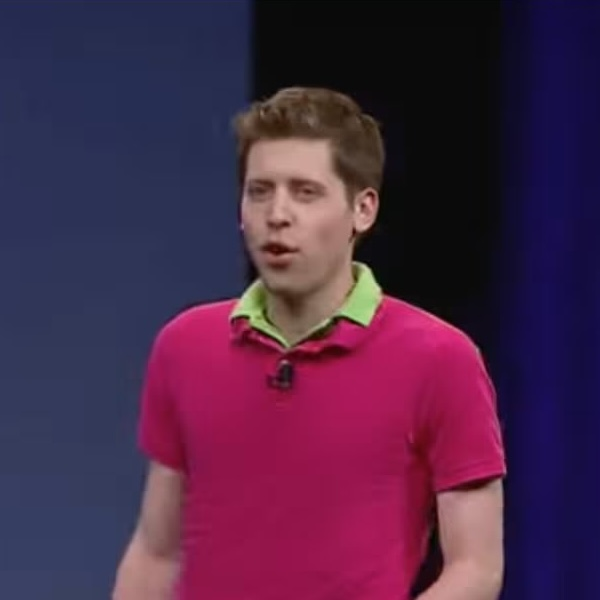
\includegraphics[alt={./sam altman double polo},height=1in]{./sam-altman-double-polo.jpg}

\includegraphics[alt={./dario amodei},height=1in]{./dario-amodei.jpg}
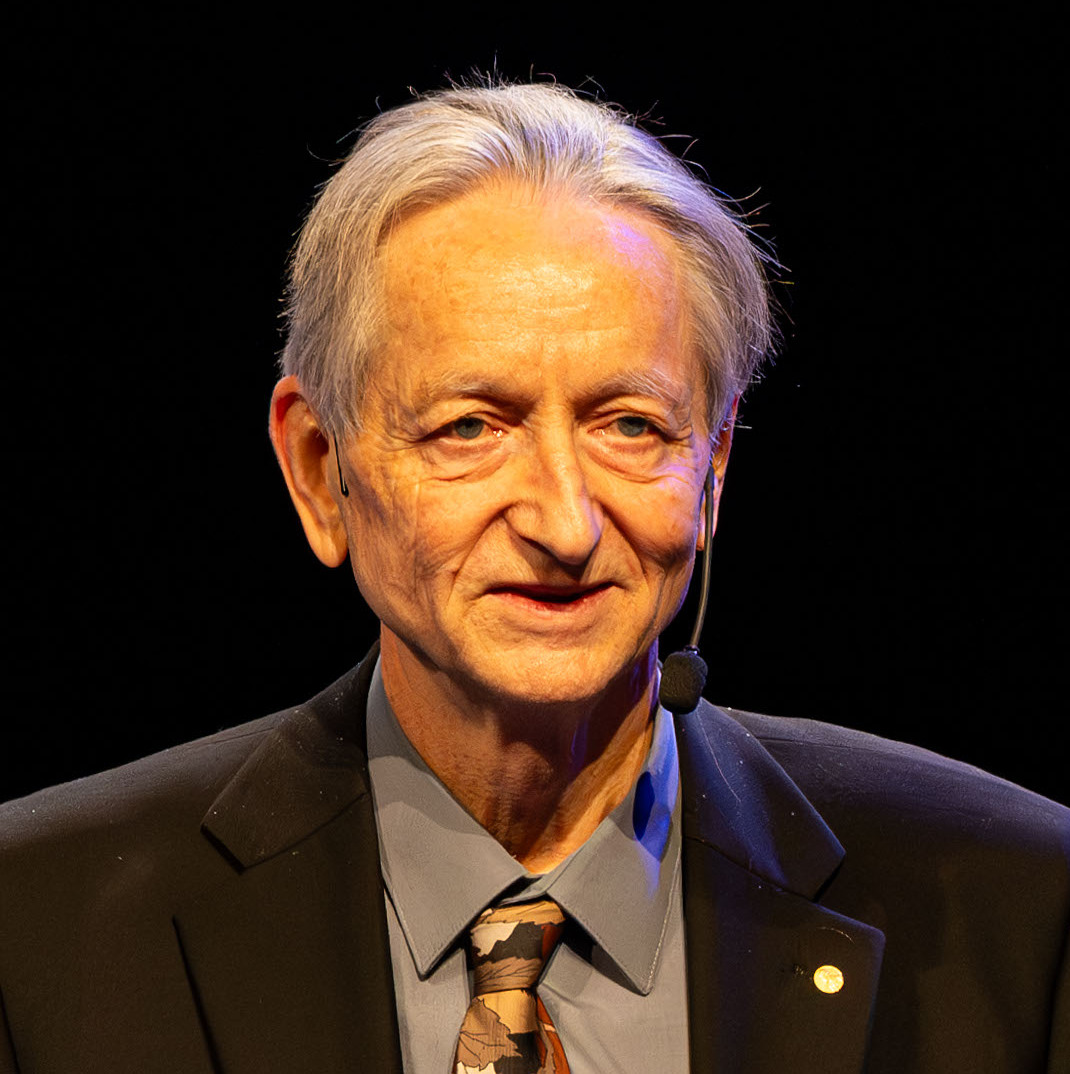
\includegraphics[alt={./geoff hinton},height=1in]{./geoff-hinton.jpg}
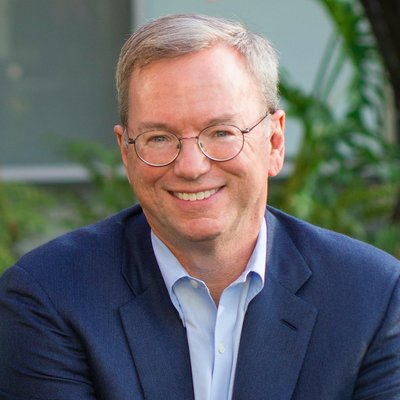
\includegraphics[alt={./eric schmidt},height=1in]{./eric-schmidt.jpg}
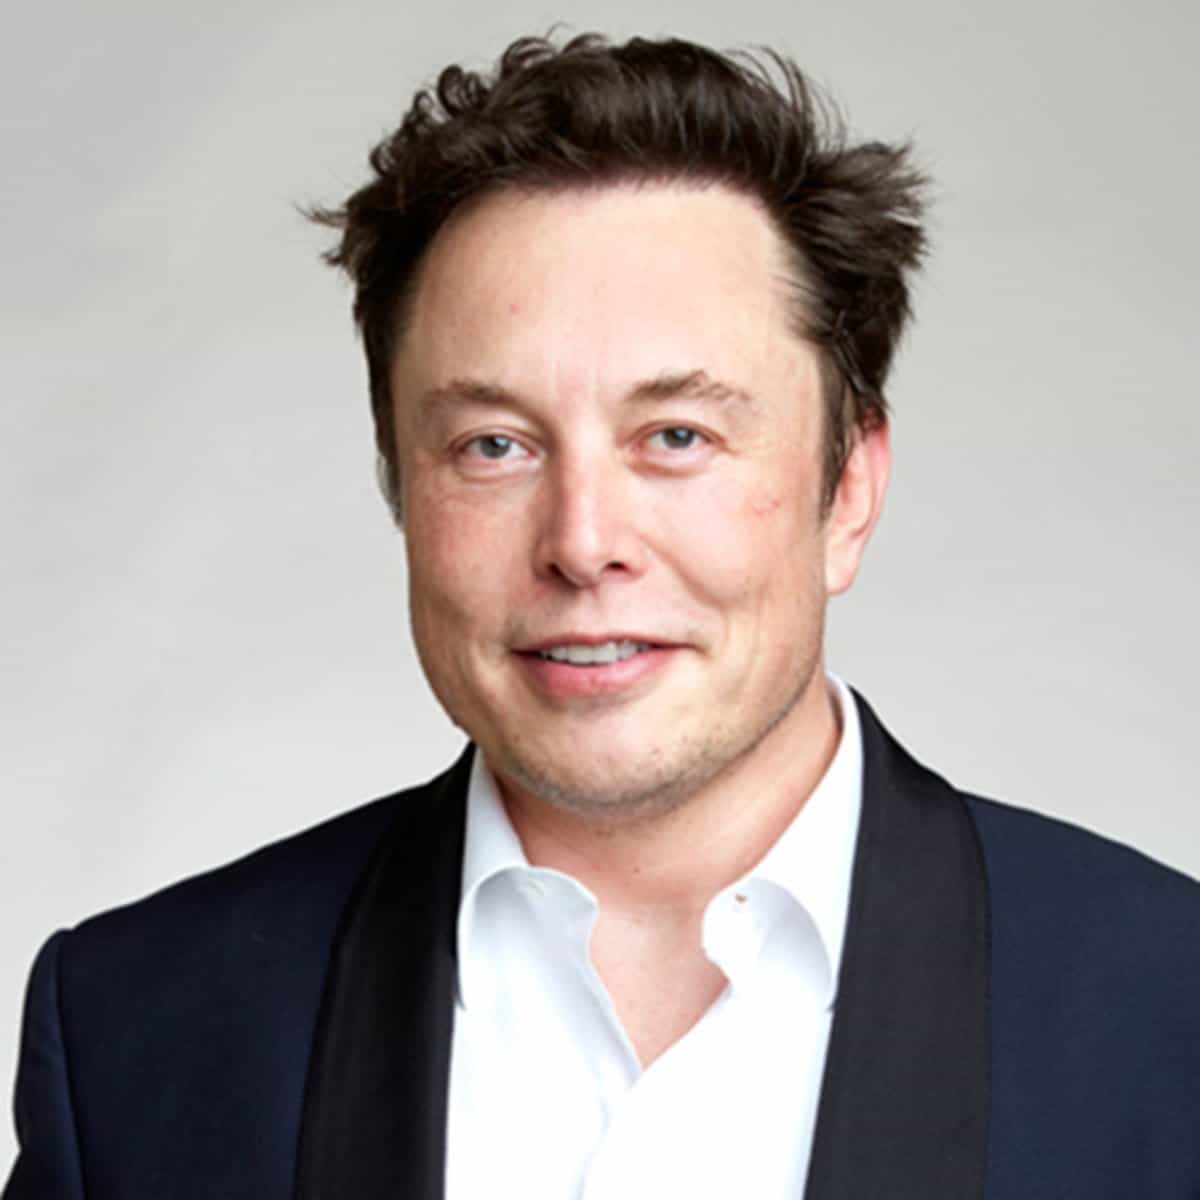
\includegraphics[alt={./elon musk},height=1in]{./elon-musk.jpg}
</center>


To be fair, there are many, many people who are wrong about AI.  But you probably recognize these guys.

\begin{itemize}
\item The emergence of "human-level AI" has been "just a few years away" since 1956.  All of these predictions have been wrong.
\end{itemize}
\section{We are decades, perhaps centuries away from "solving" AI.}
\label{sec:org14e2693}

\begin{itemize}
\item AI is immature.
\item Currently, unfortunately, overhyped.
\end{itemize}


See my advisor's advisor's dated predictions:

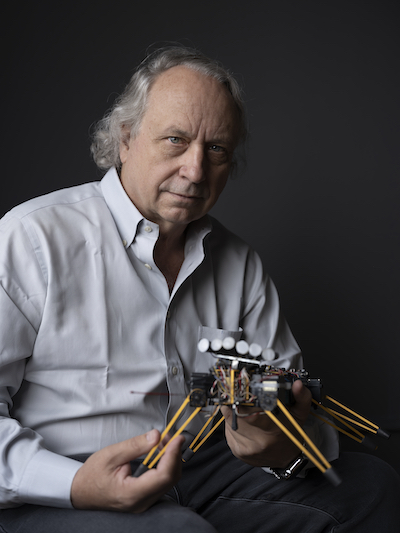
\includegraphics[alt={rodney brooks},height=1in]{rodney-brooks.jpg}

\url{https://rodneybrooks.com/my-dated-predictions/}
\section{Why does it matter that the aforementioned hypers are wrong?}
\label{sec:org383a35b}

Most of the truly groundbreaking discoveries in AI are yet to be made.

\vspace{.25in}

\LARGE{This makes AI exciting!}


\begin{itemize}
\item Many AI courses focus on \textbf{the current thing}, e.g.,  statistical machine learning, and neural networks.
\item This course covers the full spectrum of AI so that you're ready to spot and develop promising new directions.

\begin{itemize}
\item We'll spend little time on machine learning, and barely touch on neural networks.

\begin{itemize}
\item We have entire courses for those subjects!
\end{itemize}
\end{itemize}
\end{itemize}
\section{What is AI?}
\label{sec:org145d54e}





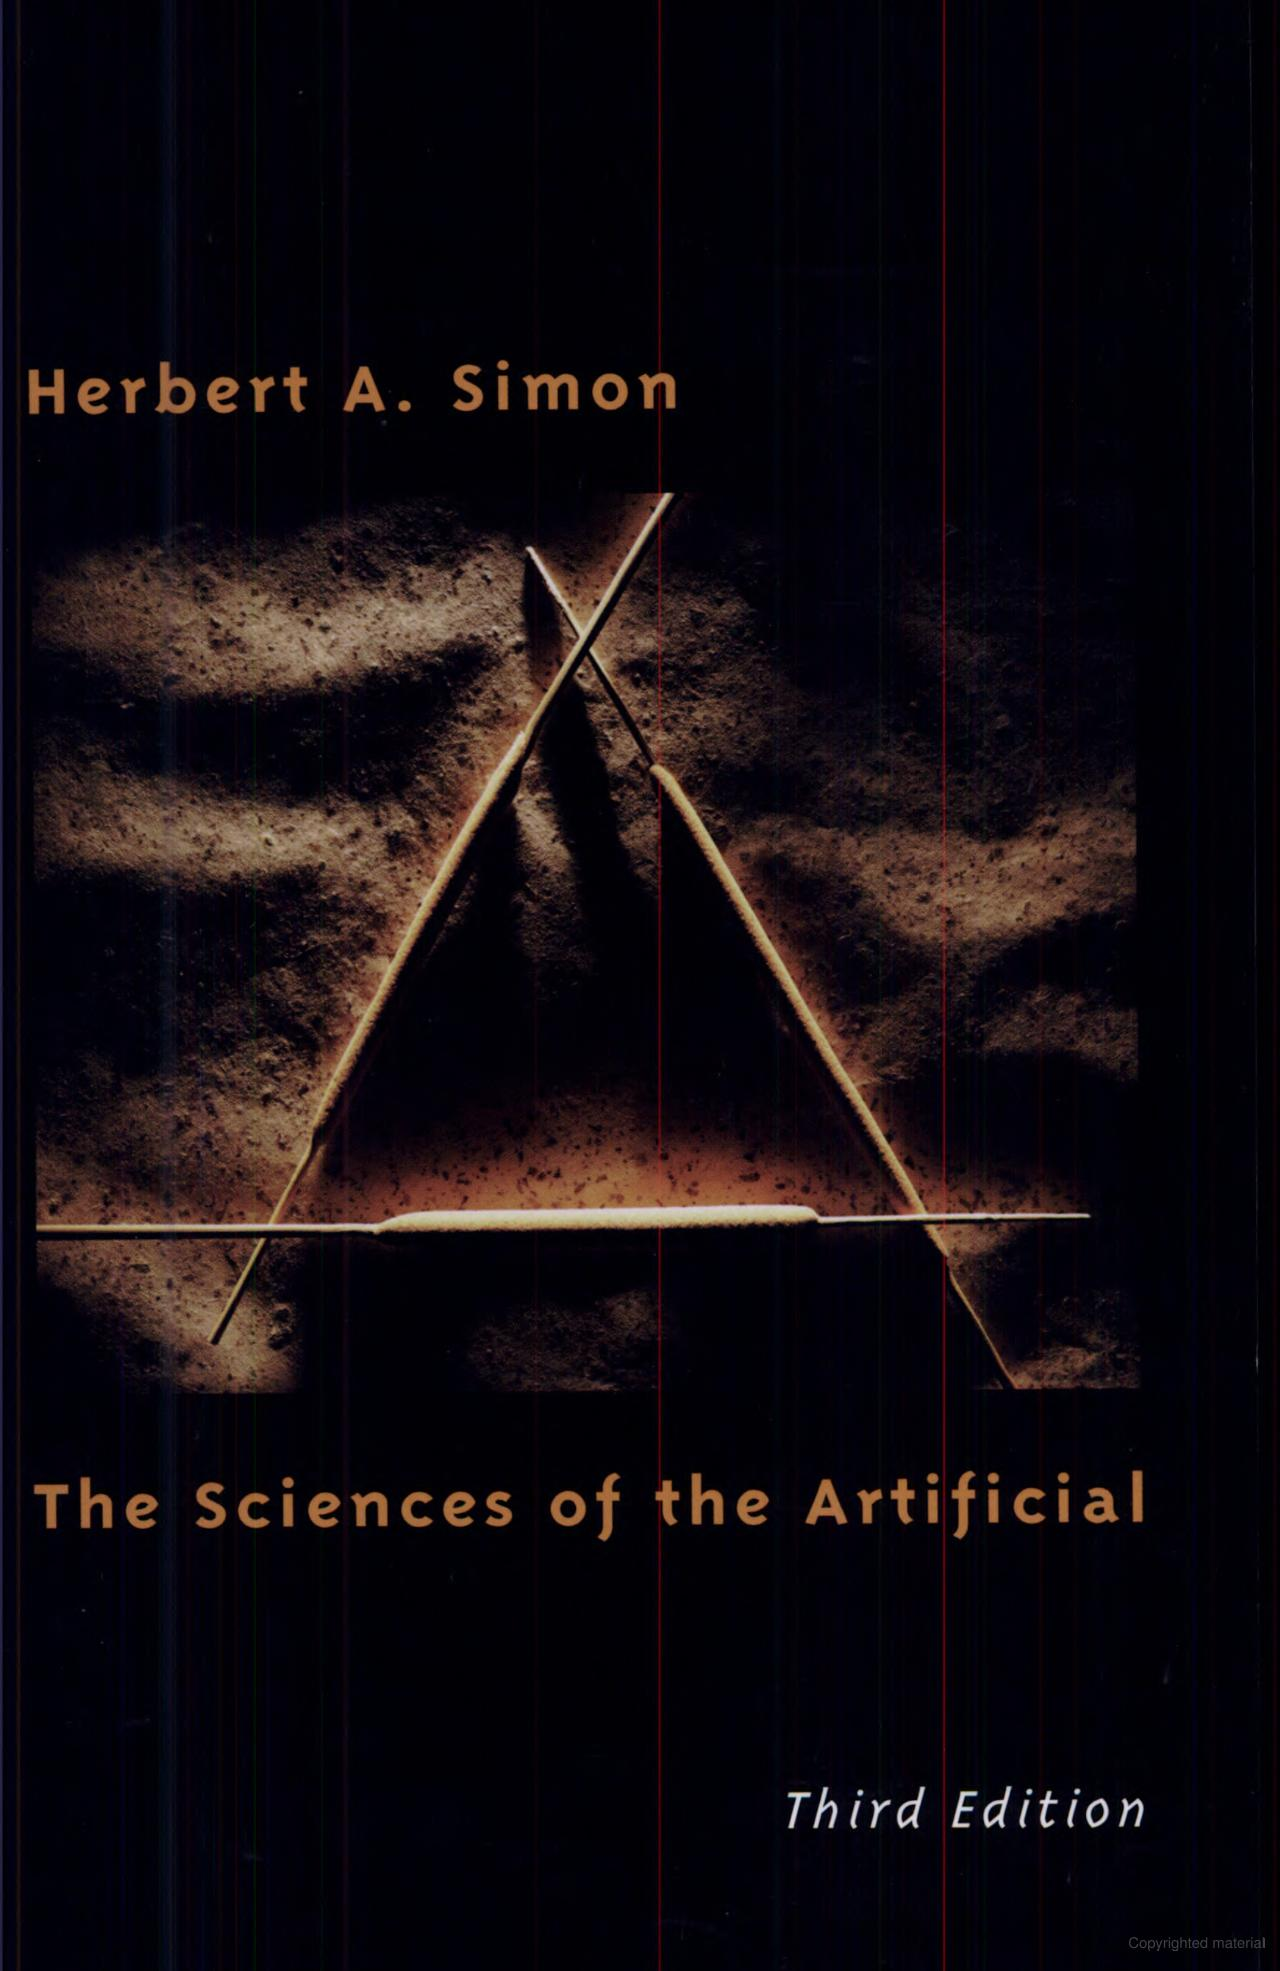
\includegraphics[alt={./simon1996sciences cover},height=1in]{./simon1996sciences-cover.jpg}






Artificial

\begin{itemize}
\item Man-made.  Synthetic.
\end{itemize}

Intelligence

\begin{itemize}
\item Problem solving
\item Reasoning
\item Decision making
\item Learning
\end{itemize}

Rationality

\begin{itemize}
\item Doing the right thing.
\end{itemize}




{[}\textsuperscript{simon1996sciences}]: \url{https://mitpress.mit.edu/9780262691918/the-sciences-of-the-artificial/}
\section{Four Approaches to AI}
\label{sec:org57e774a}

Decompose AI into thinking and acting, and define standards of performance as fidelity to humans and quantitative rationality.


\begin{tabular}{lr|cc}\\
     &          & \multicolumn{2}{c}{Standard} \\
     &          & Humanly  & Rationally \\\hline
Mode & Acting   & Acting humanly & Acting rationally \\
     & Thinking & Thinking humanly & Thinking rationally \\
\end{tabular}
\section{Acting humanly}
\label{sec:orgf133b27}

Turing test

\begin{itemize}
\item Natural language processing
\item Knowledge representation
\item Automated reasoning
\item Machine learning
\end{itemize}

Total Turing test

\begin{itemize}
\item Computer vision
\item Robotics
\end{itemize}

Nobody cares about Turing tests.
\section{Rationality}
\label{sec:org5d46155}

"Doing the right thing."

\begin{itemize}
\item Acting rationally - goal maximizing behavior

\begin{itemize}
\item Choosing actions which reach goals with minimal cost
\item Choosing actions which maximize a payoff relative to other agents
\item Choosing actions which maximize long-term expected reward
\end{itemize}

\item Thinking rationally - "laws of thought"

\begin{itemize}
\item Logic
\item Probabilistic inference
\end{itemize}
\end{itemize}


\begin{quote}
Thinking is nothing more than acting in an imagined space.
\end{quote}
\begin{quote}

\end{quote}
\begin{quote}
-- Konrad Lorenz via Bernhard Schölkopf
\end{quote}
\section{Foundations of AI}
\label{sec:org5e46072}

\begin{itemize}
\item Philosophy
\item Mathematics
\item Neuroscience
\item Psychology
\item Computer Engineering
\item Control theory and cybernetics
\item Linguistics
\end{itemize}

Such a rich tapestry!
\section{Philosophy}
\label{sec:orgd1ec2fc}

\begin{itemize}
\item Can formal rules be used to draw valid conclusions?
\item How does the mind arise from a physical brain?
\item Where does knowledge come from?
\item How does knowledge lead to action?
\end{itemize}
\section{Mathematics}
\label{sec:org9d101a4}

\begin{itemize}
\item What are the formal rules to draw valid conclusions?
\item What can be computed?
\item How do we reason with uncertain information?

\item Logic
\item Probability and statistics
\item Algorithms, computability and complexity
\item Optimization
\end{itemize}
\section{Economics}
\label{sec:orgfb692c9}

Acting rationally

\begin{itemize}
\item How should we make decisions in accordance with our preferences?
\item How should we do this when others may not go along?
\item How should we do this when the payoff may be far in the future?
\end{itemize}
\section{Neuroscience}
\label{sec:org3a98696}

How do brains process information?

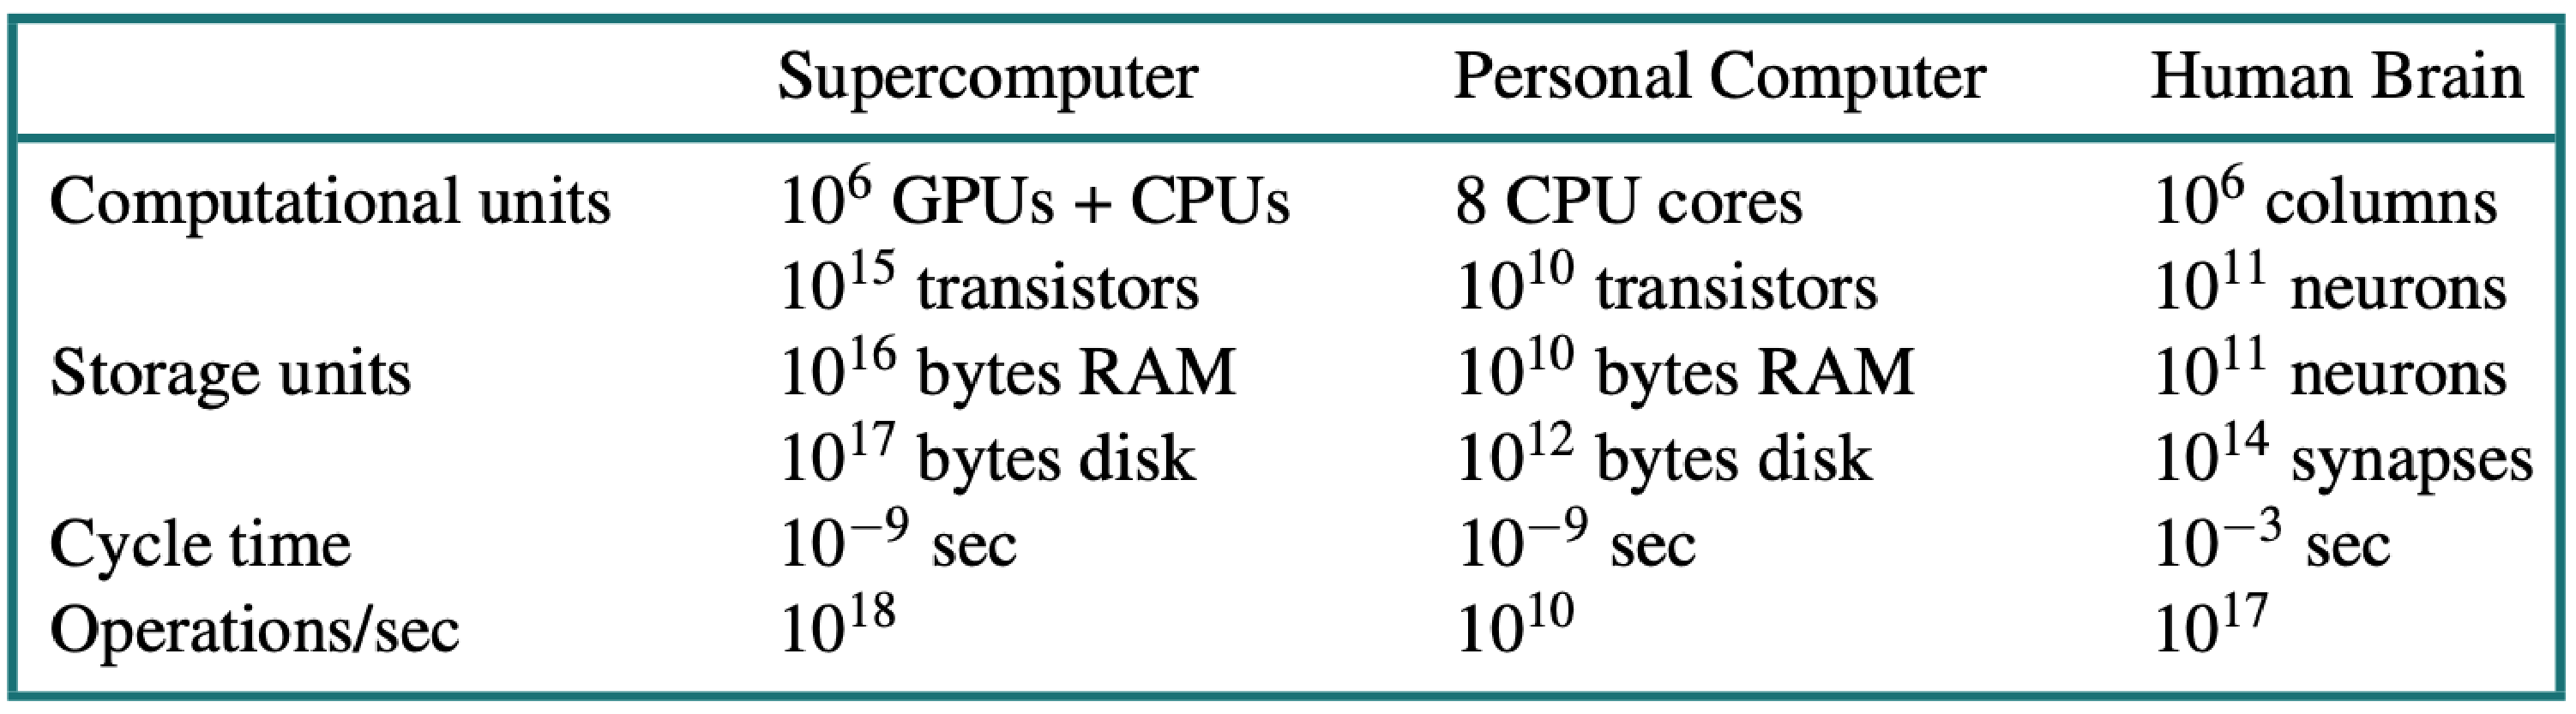
\includegraphics[alt={./aima fig 01_02 computers vs brains},height=1in]{./aima-fig-01_02-computers-vs-brains.pdf}
\section{Psychology}
\label{sec:orgb73da20}

How do humans and animals think and act?

\begin{itemize}
\item Cognitive modeling
\item Behaviorism

\begin{itemize}
\item Operant conditioning
\item "Reinforcement learning"
\end{itemize}
\end{itemize}
\section{Computer Engineering}
\label{sec:org64f1542}

How can we build an efficient computer?

\begin{itemize}
\item High performance computing

\begin{itemize}
\item Today's LLMs take years of compute time to train.
\end{itemize}

\item Quantum computing
\end{itemize}

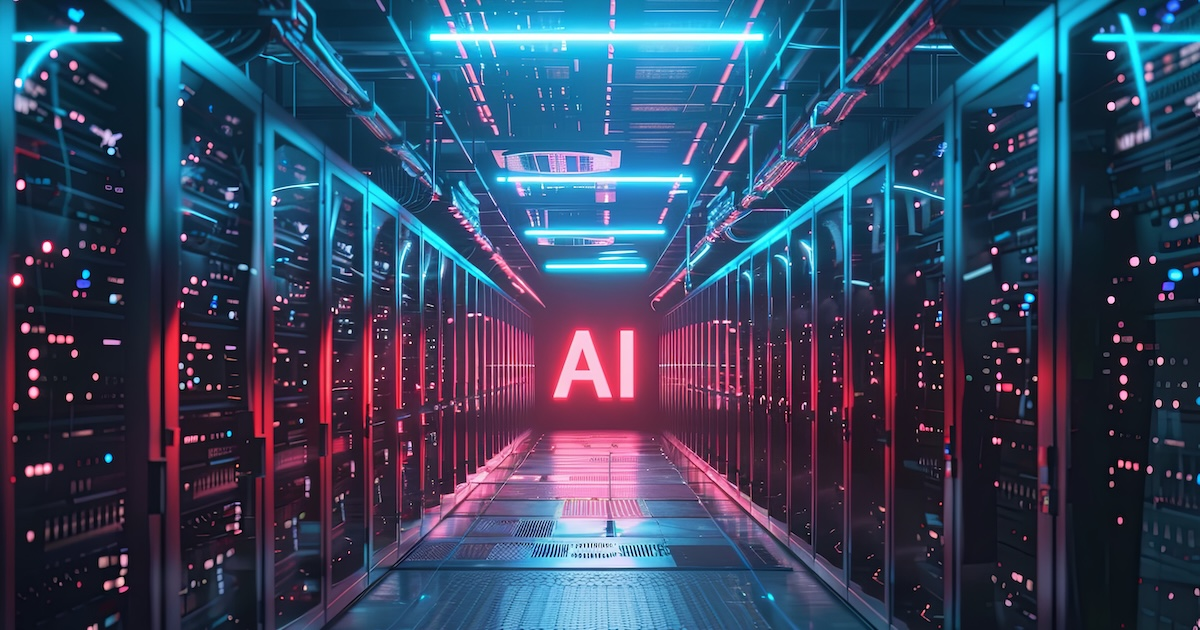
\includegraphics[alt={ai data center},height=1in]{ai-data-center.jpg}
\section{Control theory and cybernetics}
\label{sec:orgc9111a7}

How can artifacts operate under their own control?

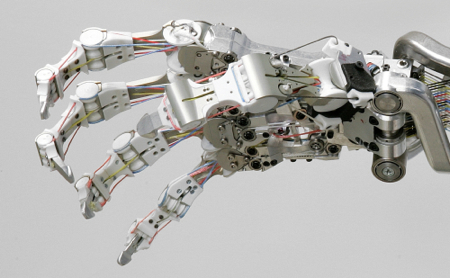
\includegraphics[alt={robot hand},height=1in]{robot-hand.jpg}
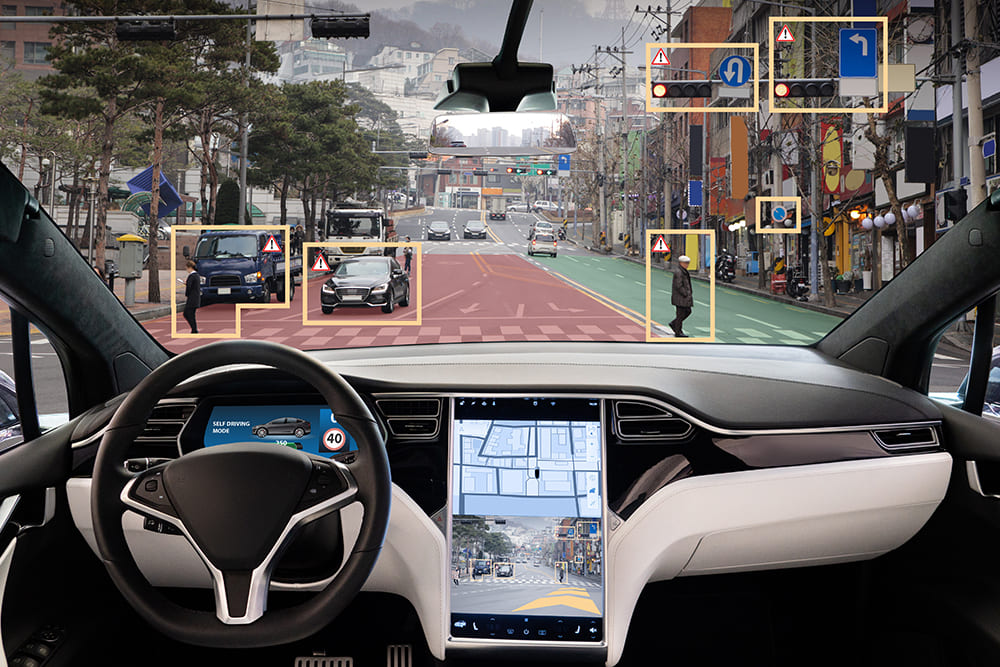
\includegraphics[alt={self driving car},height=1in]{self-driving-car.jpg}

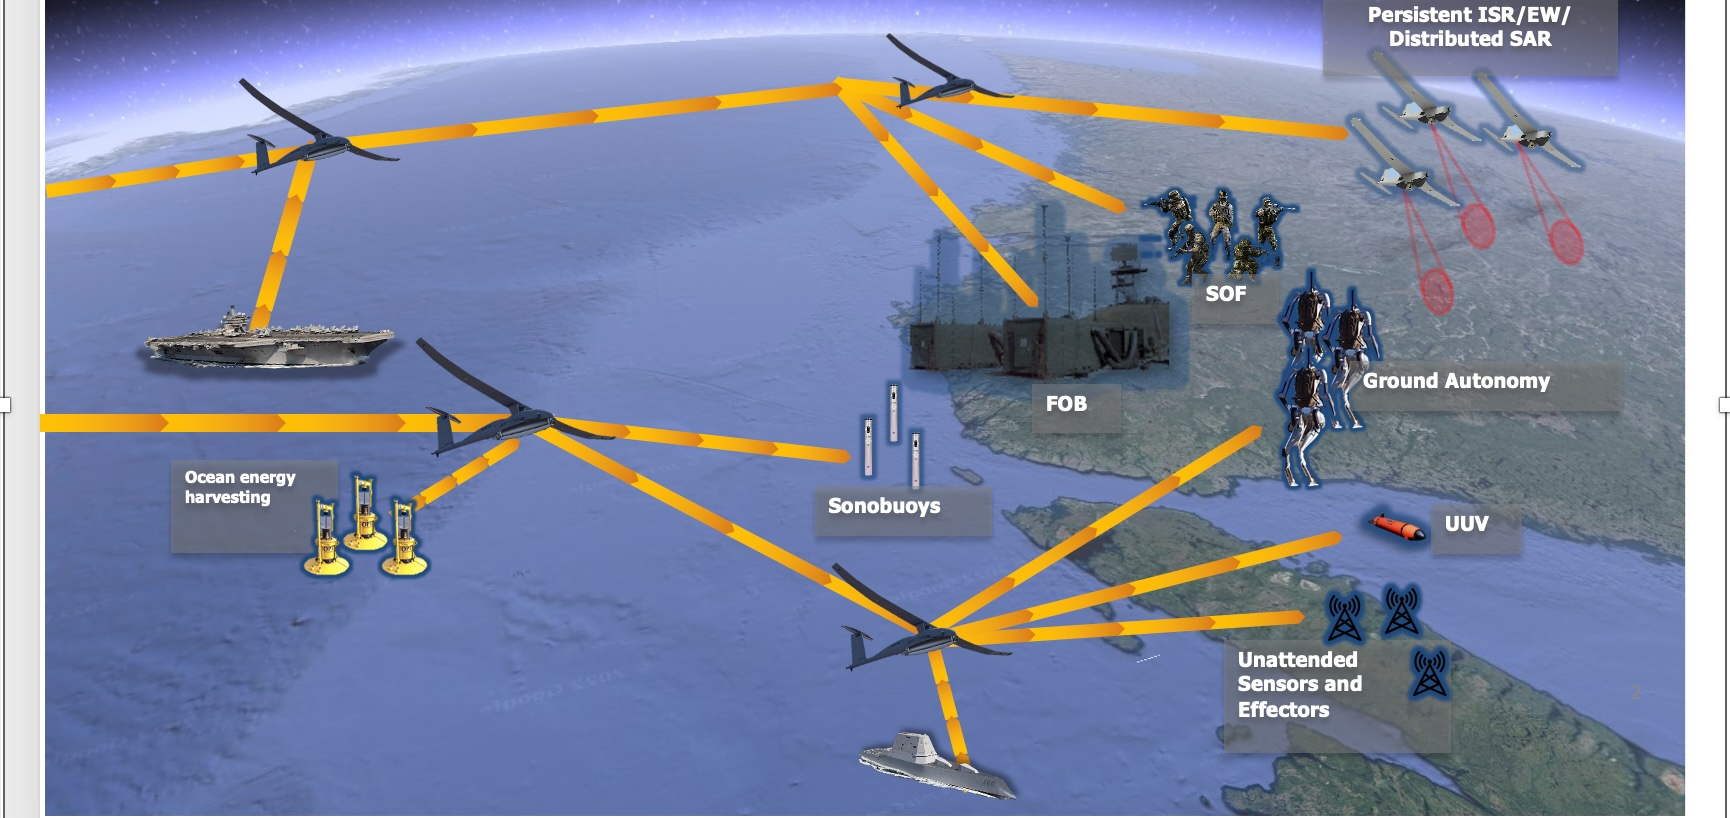
\includegraphics[alt={Power Relay 6},height=1in]{Power-Relay-6.jpg}

\href{https://www.darpa.mil/research/programs/power}{DARPA POWER Program}
\section{Impact of AI}
\label{sec:org9f86b77}

Turing award winners:

\begin{itemize}
\item Marvin Minsky (1969)
\item John McCarthy (1971)
\item Allen Newell and Herbert Simon (1975)
\item Ed Feigenbaum and Raj Reddy (1994)
\item Judea Pearl (1994)
\item Yoshua Bengio, Geoffrey Hinton, and Yann LeCun (2019)
\item Rich Sutton and Andrew Barto (2024)
\end{itemize}

AI lament: once an AI problem is solved, it's no longer considered AI.
\section{History of AI}
\label{sec:orgbf2cbe4}

\begin{itemize}
\item MucCulloch, Pitts, Hebb (1943-1949)

\begin{itemize}
\item Perceptrons
\item Hebbian learning
\end{itemize}

\item 1956 Dartmouth AI Workshop

\begin{itemize}
\item Organized by John McCarthy, Marvin Minsky, Claude Shannon, Nathaniel Rochester
\item Attended by Allen Newell and Herbert Simon from Carnegie Tech, Trenchard More from Princeton, Arthur Samuel from IBM, and Ray Solomonoff and Oliver Selfridge from MIT
\end{itemize}

\item Symbolic AI (1952-1969) -- "clever Lisp programs"

\item First AI Winter (1966-1973)

\begin{itemize}
\item Lighthill report (Lighthill, 1973) -- British government ended most AI funding
\end{itemize}

\item Expert Systems (1969-1986)

\item Second AI Winter (1986)

\begin{itemize}
\item Experts systems failed to deliver on their inventors' promises.
\item Knowledge acquisition bottleneck.
\item Adaptability, brittleness.
\end{itemize}
\end{itemize}
\section{Modern AI}
\label{sec:org91223d2}

\begin{itemize}
\item Return of neural networks (1986-present)

\begin{itemize}
\item Symbolism vs Connectionism
\item Geoff Hinton, et. al.
\end{itemize}

\item Probabilistic reasoning and machine learning (1987-present)

\begin{itemize}
\item Neats vs scruffies
\item "Physics envy"
\end{itemize}

\item Big data (2001-present)

\begin{itemize}
\item Large data sets -- don't fit on a single machine
\end{itemize}

\item Deep learning (2011-present)

\begin{itemize}
\item You may have heard of it?
\end{itemize}
\end{itemize}
\section{Future of AI}
\label{sec:orgaacbcda}




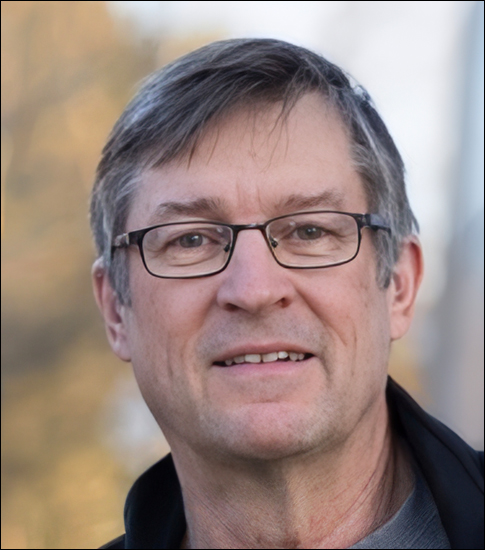
\includegraphics[alt={andrew barto},height=1in]{andrew-barto.jpg}

\href{https://people.cs.umass.edu/\~barto/}{Andrew Barto}




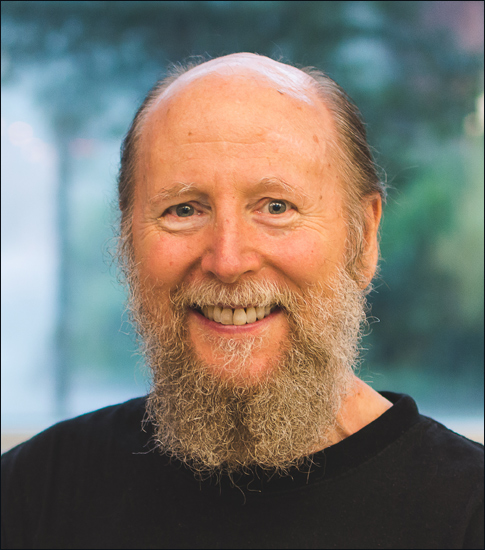
\includegraphics[alt={rich sutton},height=1in]{rich-sutton.jpg}
\href{http://incompleteideas.net/}{Rich Sutton}




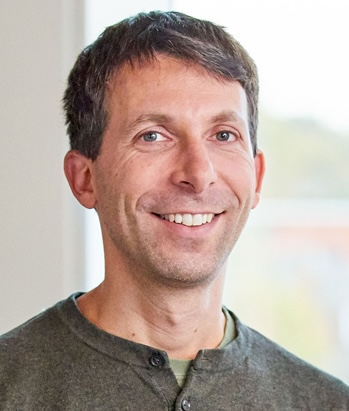
\includegraphics[alt={david silver},height=1in]{david-silver.jpg}
\href{https://davidstarsilver.wordpress.com/}{David Silver}




\href{https://storage.googleapis.com/deepmind-media/Era-of-Experience\%20/The\%20Era\%20of\%20Experience\%20Paper.pdf}{The Era of Experience}
\end{document}
